\section{事例仿真}\label{sec:evt_simulation}
%物理分析的一项重要目标是比较高能对撞的观测数据和某些假设或者预测模型,包括某些感兴趣的物理过程以及相应本底过程。
%通常情况下,可用的观测数据数量有限,不足以提供足够精度去描述需要的物理过程,尤其是当该物理过程截面本身很小时。
%所以,对标准模型物理过程以及新物理模型进行仿真是非常有必要的,可以提供大量的仿真事例用来理解与研究。
物理分析的一项重要目标是验证或排除理论预测,在对撞实验中,理论预测需要与观测数据进行比较,
为实现这一目的,需要对理论模型进行仿真。同时仿真事例也可用来理解本底组成和新信号运动学分布。

ATLAS的仿真是包括事例产生和探测器模拟的多步骤过程。
一个典型的质子质子-对撞过程如图~\ref{fig:evt_egen_chain}所示,一般关心的是携带大动量的部分子的碰撞,即硬散射过程,而后衰变,部分子簇射以及强子化得到稳定粒子,这些都通过蒙特卡罗事件产生子(Monte-Carlo generator)模拟\cite{BUCKLEY2011145}。最后,模拟稳定粒子与探测器的相互作用。
\begin{figure}
\centering
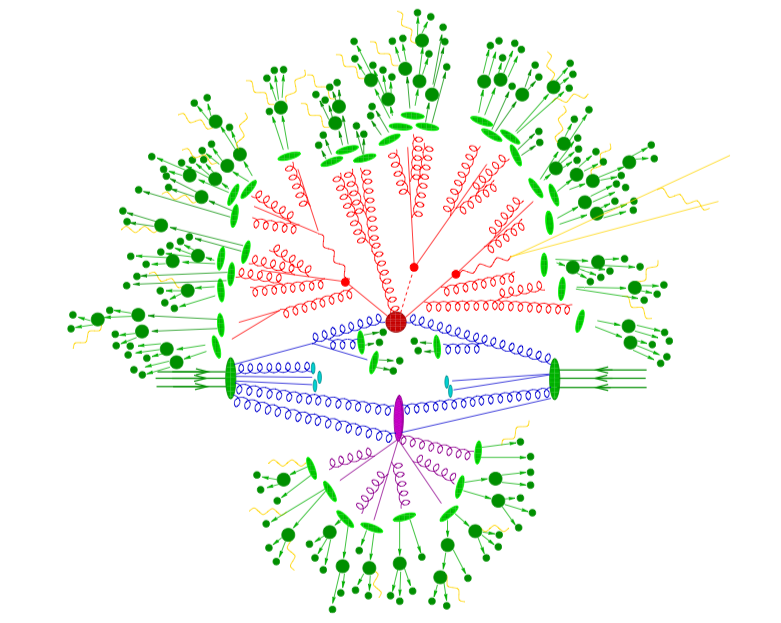
\includegraphics[width=0.75\textwidth]{fig/evt_egen_chain.png}
\caption{产生子中$t\bar{t}h$事例演化过程\cite{Gleisberg:2008ta}。首先携带大动量的硬散射过程发生(大红色圆),随后$t$和$h$衰变(小红色圆),衰变产物发生QCD硬辐射(红色);除硬散射之外,次要散射(由参与硬散射之外的部分子参与)也可能发生(紫色);最后辐射到一定低能量时,强子化过程发生(浅绿),强子化产物衰变到稳定粒子(深绿)。光子辐射可在任一阶段发生(黄色)。}
\label{fig:evt_egen_chain}
\end{figure}
\begin{itemize}
  \item 整合所仿真的物理过程的相空间(运动学,自旋),在一定的QCD或者QED微扰展开级数下计算并模拟硬散射过程(Matrix element)。
  \item 利用专用程序模拟硬散射过程的部分子的初态和末态辐射胶子以及紧接的部分子簇射过程(PS),在这一般是使用微扰QCD来模拟粒子级联,通常能到次级对数精度(NLL),这个过程直到微扰QCD不再
  适用的尺度$\Lambda_{\text{QCD}}\approx200$MeV才停止。类似PS,QED过程的辐射光子利用等价的数学框架模拟。
  \item 强子化过程不依赖于初始的物理过程,即Matrix element,它不能使用微扰QCD论,目前从第一性原理出发也未能理解,所以一般通过基于实验数据的唯象模型描述,所使用的方法
      在不同的软件环境中有不同的实现。
   \item 仿真\texttt{underlying event} (UE)。UE代表了碰撞质子中未参与硬散射过程的部分子的强子化,或者它们之间的相互作用,它们可以是微扰QCD尺度,也可以在非微扰尺度。同样地。
   导致\pileup 的\texttt{minimum bias}事件也会叠加在硬散射事例中。
   \item 利用GEANT4软件\cite{AGOSTINELLI2003250}模拟前面步骤产生的稳定粒子与探测器的相互作用,探测器的几何形状与材料分布都会考虑\cite{Aad2010-atlas-simu}。这个步骤是是整个ATLAS实验耗费计算资源最多的一环,
     所以对某些过程使用所谓的快速模拟技术(fast simulation)\cite{Lukas:2012kua}以节省计算资源和加快模拟过程。
    \item 探测器着火点被复现并数字化,而后进行与对撞数据完全一样的事例重建过程,并且以相同的文件格式存储。在这过程中,也对触发决策进行模拟。
 \end{itemize}

 如前所述,仿真样本的重建效率,鉴别效率,触发效率和能量刻度以及能量校准都会乘上一定的修正因子使之与真实数据匹配,需要注意的是,pileup仿真强烈依赖假设的对撞条件。
